\section{Обзор литературы}
\label{sec:domain}

В данном разделе будет произведён обзор предметной области задачи, решаемой в рамках курсового проекта; рассмотрены вопросы о способах обнаружения движений, методы анализа и алгоритмы обнаружения лиц и рассмотрены библиотеки обработки визуальной информации.

\subsection{Обнаружение движений}
\label{sub:domain:motion_detect}

Видеоданные проверяются на наличие определенного условия. Например, обнаружение возможных неправильных клеток или тканей в медицинских изображениях. Обнаружение, основанное на относительно простых и быстрых вычислениях, иногда используется для нахождения небольших участков в анализируемом изображении, которые затем анализируются с помощью приемов, более требовательных к ресурсам, для получения правильной интерпретации. Существует несколько специализированных задач, основанных на распознавании текстов, например: Поиск изображений по содержанию: нахождение всех изображений в большом наборе изображений, которые имеют определенное содержание. Содержание может быть определено различными путями, например, в терминах схожести с конкретным изображением (найдите мне все изображения похожие на данное изображение), или в терминах высокоуровневых критериев поиска, вводимых как текстовые данные (найдите мне все изображения, на которых изображено много домов, которые сделаны зимой и на которых нет машин).Оценка положения: определение положения или ориентации определенного объекта относительно камеры. Примером применения этой техники может быть содействие руке робота в извлечении объектов с ленты конвейера на линии сборки~\cite{gorelik_2004}.
Оптическое распознавание знаков: распознавание символов на изображениях печатного или рукописного текста, обычно для перевода в текстовый формат, наиболее удобный для редактирования или индексации (например, ASCII).

Рассмотрим подробнее методы обнаружения движений

\subsubsection{Межкадровая разность. }
\label{sub:domain:motion_detect:frames_diff_method}
Вычисление межкадровой разности является распространённым методом первичного обнаружения движения, после выполнения которого можно определить присутствует ли в потоке кадров движение~\cite{md_1998}. Алогоритм вычисления межкадровой разности выглядит следующим образом: на вход поступают два видеоряда, представляющие собой две последовательности
байт. Производится вычисление попиксельных межкадровых разностей по следующей схеме
\begin{equation}\label{eq:frames_diff}
d_t\left(x,y\right) = I_t\left(x,y\right) - I_{t-1}\left(x,y\right)
\end{equation}
Разность сравнивается с заданным порогом. В результате сравнения формируется двоичная маска:

\begin{equation}\label{eq:fr_diff_bitmask}
m_t\left(x,y\right) = 
\begin{cases}
 & 0, {d}_{t}\left(x,y\right)<T  \\ 
 & 1, {d}_{t}\left(x,y\right)>T
\end{cases}
\end{equation}

где $m_t$ --- значение t-го элемента маски, T --- порог сравнения, иногда называемый также порогом или уровнем чувствительности.

Однако такой подход даёт достаточно грубую оценку, приводя к наличию неизбежной ложной реакции детектора на шум регистрирующей аппаратуры, смену условий освещения, лёгкое качание камеры и пр. Таким образом, видеокадры должны быть предварительно обработаны перед вычислением разности между ними. Например, преобразование цветов изображения к серой гамме даст большую скорость выполнения операций~\cite{soyfer_1996}.

Для сравнения могут быть использованы соседние кадры или текущий и базовый кадр (базовый кадр содержит фон).

\subsubsection{Метод вычитания фона. }
\label{sub:domain:motion_detect:back_remove_method}
Суть алгоритма заключается в разделении изображения на фоновую область и передний план~\cite{fisher_2002}.
Существует множество алгоритмов метода вычитания фона, но большинство имеют примерно одинаковую структуру.
Основными этапами данного алгоритма являются предобработка, моделирование фона, обнаружение движения и постобработка.

Типовая схема реализации метода вычитания фона представлена на рисунке~\ref{fig:back_rem_scheme}.
\begin{figure}[ht]
\centering
    \centering
    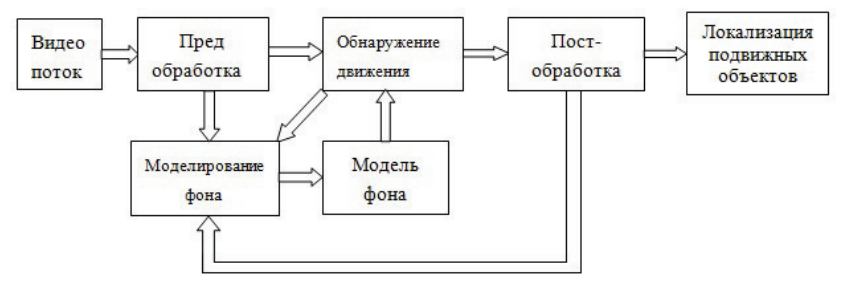
\includegraphics[scale = 0.65]{back_remove.png}  
  \caption{Схема обнаружения подвижных объектов.}
  \label{fig:back_rem_scheme}
\end{figure}

Моделирование фона.

Фон можно использовать фиксированный - заранее подготовленный кадр. Для всех остальных кадров применяется порог к модулю разности текущего и сохраненного изображения по каждому пикселю.
 
Для моделирования фона чаще используется метод усреднения. Модель фона будет среднее от первых n кадров:
\begin{equation}
	BG\left(x,y\right) = \frac{1}{n}\cdot \sum_{i=1}^{n}I_i\left(x,y \right )
\end{equation}

Для того чтобы алгоритм был устойчив к изменению фона, необходимо обновлять фон в течении всего времени на основе начальной модели фона~\cite{fsdg_2010}.	

\subsection{Обнаружение лиц}
\label{sub:domain:face_detect}

По сути, отслеживание и распознавание лиц является практическим применением теории распознавания образов, в задачу которого входит автоматическая локализация лица на фотографии или видеопотоке и, в случае необходимости, идентификация персоны по лицу. В настоящее время функцию идентификации людей на фотографиях уже активно используют в программном обеспечении для управления фотоальбомами (Picasa, iPhoto и др.)~\cite{face_wiki}

\subsubsection{Метод Виолы-Джонса. }
\label{sub:domain:face_detect:viola_jones_method}
В настоящее время метод Виолы"--~Джонса является самым популярным методом для поиска области лица на изображении в силу своей высокой скорости и эффективности. В основе метода Виолы"--~Джонса по поиску лица лежат идеи: интегральное представление изображения по признакам Хаара, метод построения классификатора на основе алгоритма адаптивного бустинга, и метод комбинирования классификаторов в каскадную структуру~\cite{fd_2012}. Эти идеи позволяют осуществлять поиск лица в режиме реального времени.
	
Признак Хаара состоит из смежных прямоугольных областей. Эти области позиционируются на изображении, далее происходит суммирование интенсивности пикселей в областях, затем между суммами вычисляется разность. Значение полученной разности и является значением определенного признака, определенного размера, определенным образом расположенного на изображении. На рисунке~\ref{fig:haar_features} представлены граничные, центральные и линейные признаки Хаара. Рисунок~\ref{fig:haar_using} демонстрирует пример использования признаков Хаара. На пример, для всех изображений, область в районе глаз темнее, чем область в районе щек. Следовательно, общим признаком Хаара для лиц является 2 смежных прямоугольных региона, лежащих на глазах и щеках.

На этапе обнаружения в методе Виолы"--~Джонса используется окно, определенного размера, которое движется по изображению. Признак Хаара рассчитывается для каждой области изображения, над которой проходит окно. Наличие или отсутствие предмета в окне определяется разницей между значением признака и обучаемым порогом. Поскольку признаки Хаара мало подходят для обучения или классификации, для описания объекта с достаточной точностью необходимо большее число признаков. Поэтому в методе Виолы"--~Джонса признаки Хаара организованы в каскадный классификатор.

\begin{figure}[ht]
\centering
    \centering
    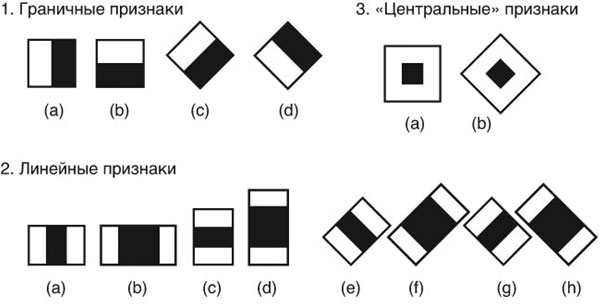
\includegraphics[scale = 0.5]{haar_features.jpg}  
  \caption{Признаки Хаара}
  \label{fig:haar_features}
\end{figure}
\begin{figure}[ht]
\centering
    \centering
    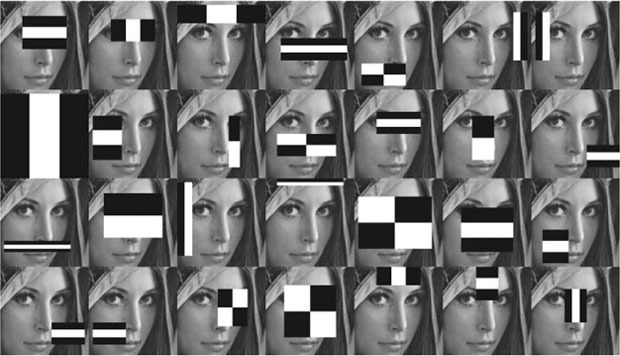
\includegraphics[scale = 0.4]{haar_using.jpg}  
  \caption{Примеры использования признаков Хаара.}
  \label{fig:haar_using}
\end{figure}

Преимущество использования признаков Хаара является наибольшая, по сравнению с остальными признаками, скорость. При использовании интегрального представления изображения, признаки Хаара могут вычисляться за постоянное время.

Методу Виолы"--~Джонса присуща высокая вероятность точного обнаружения лица, даже при наблюдении объекта под небольшим углом, примерно до $30^\circ$. Но при большем угле наклона вероятность обнаружения лица резко падает. В стандартной реализации метода указанная особенность не позволяет обнаруживать лицо человека, повернутое под произвольным углом, что в значительной мере затрудняет или делает невозможным использование данного метода в современных системах.

\subsubsection{Метод главных компонент. }
\label{sub:domain:face_detect:main_component_method}
Главная идея этого метода состоит в представлении изображений лиц людей в виде набора главных компонент изображений, называемых "собственные лица" (Eigenfaces). Полезным свойством собственных лиц является то, что изображение, соответствующее каждому такому компоненту имеет лицеподобную форму, как представлено на рисунке~\ref{fig:vectors} Вычисление главных компонент основывается на вычислении собственных векторов и собственных значений ковариационной матрицы, которая рассчитывается из изображения. Сумма главных компонент, умноженных на соответствующие собственные вектора, является реконструкцией изображения~\cite{fd_2012}.
\begin{figure}[ht]
\centering
    \centering
    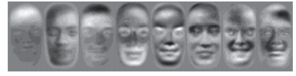
\includegraphics{vectors.png}  
  \caption{Пример изображений собственных векторов.}
  \label{fig:vectors}
\end{figure}

Для каждого изображения лица вычисляются его главные компоненты. Обычно берётся от 5 до 200 главных компонент. Остальные компоненты кодируют мелкие различия между лицами и шумами. Процесс распознавания заключается в сравнении главных компонент неизвестного изображения с компонентами всех известных изображений. При этом предполагается, что изображения лиц, соответствующих одному человеку, сгруппированы в кластеры в собственном пространстве. Из базы данных выбираются изображения кандидаты, имеющие наименьшее расстояние от входного (неизвестного) изображения.


\subsection{Обработка изображений}
\label{sub:domain:img_proc}

Для обработки изображений в ЭВМ можно использовать вычислительные мощности CPU или GPU. Обработка изображений в центральном процессоре выполняется отдельно для каждой цветовой компоненты пикселя, то есть сложность алгоритма оценивается сложностью обработки одного пикселя умноженной на общее количество компонентов в пикселе и умноженной на количество пикселей в изображении. К этому можно добавить влияние скорости передачи информации из памяти в процессор и обратно. Для решения данной задачи в процессор были добавлены инструкции по обработке пакетной мультимедийной информации --- SIMD инструкции.

Расширенный  набор  команд MMX впервые  появился  в  процессорах Intel Pentium 
MMX и с тех пор поддерживается всеми более современными процессорами фирмы Intel, 
а также процессорами фирмы AMD, начиная с AMD K6. Инструкции SSE появились 
в процессорах Intel Pentium III. Эти расширения стандартных наборов команд процессоров 
6-го поколения позволяют обрабатывать одной инструкцией сразу несколько пар чисел. 
Такая  пакетная  обработка  может  дать  значительное  ускорение  работы  алгоритма,  когда 
необходимо много раз выполнять одни и те же операции над различными данными. Это 
как раз имеет место при обработке изображений. 

Блок  команд MMX использует 64-битные MMX-регистры,  большинство  команд 
расширения SSE выполняются над содержимым 128-битных регистров блока XMM.  Соответственно это позволяет эффективно обрабатывать 1-2 пикселя за раз при использовании команд блока MMX и до 4 пикселей при использовании SSE. Заметим, что, применяя обычные операции, мы могли обрабатывать всего одну из 3-х компонент 
цвета пикселя за раз. 

Кроме того, в блоке команд SSE есть удобные инструкции, позволяющие переписывать содержимое регистров MMX и XMM напрямую в память, минуя кэш. Это полезно, в том случае, если заранее известно, что содержимое регистра, переписанное в память понадобится не скоро. Использование таких операций позволяет существенно сократить накладные расходы на работу с кэш-памятью.

Хотя и описанные выше способы и позволяют в 5\--~6 раз ускорить выполнение обработки, но для больших изображений этого недостаточно. Для обработки графических данных выгоднее использовать GPU или графический процессор. Современные графические процессоры очень эффективно обрабатывают и отображают компьютерную графику. Благодаря специализированной конвейерной архитектуре они намного эффективнее в обработке графической информации, чем типичный центральный процессор. Графический процессор в современных видеоадаптерах применяется в качестве ускорителя трёхмерной графики.

Высокая вычислительная мощность GPU объясняется особенностями архитектуры. Если современные CPU содержат несколько ядер, графический процессор изначально создавался как многоядерная структура, в которой количество ядер может достигать несколько тысяч. Разница в архитектуре обусловливает и разницу в принципах работы. Если архитектура CPU предполагает последовательную обработку информации, то GPU исторически предназначался для обработки компьютерной графики, поэтому рассчитан на массивно параллельные вычисления.

Если алгоритм решения задачи может быть распараллелен на тысячи отдельных потоков, то эффективность решения такой задачи с применением GPU может быть выше, чем ее решение средствами только процессора общего назначения. Однако нельзя так просто взять и перенести решение какой-то задачи с CPU на GPU, хотя бы просто потому, что CPU и GPU используют разные команды. То есть когда программа пишется под решение на CPU, то применяется набор команд х86 (или набор команд, совместимый с конкретной архитектурой процессора), а вот для графического процессора используются уже совсем другие наборы команд, которые опять-таки учитывают его архитектуру и возможности. 

Когда стали предприниматься первые попытки реализовать неграфические вычисления на GPU, возник компилятор BrookGPU. До его создания разработчикам приходилось получать доступ к ресурсам видеокарты через графические API OpenGL или Direct3D, что значительно усложняло процесс программирования, так как требовало специфических знаний ---- приходилось изучать принципы работы с 3D-объектами (шейдерами, текстурами и т.п.). Это явилось причиной весьма ограниченного применения GPU в программных продуктах. BrookGPU стал своеобразным «переводчиком». Эти потоковые расширения к языку Си скрывали от программистов трехмерный API и при его использовании надобность в знаниях 3D-программирования практически отпала. Вычислительные мощности видеокарт стали доступны программистам в виде дополнительного сопроцессора для параллельных расчетов. Компилятор BrookGPU обрабатывал файл с кодом Cи и расширениями, выстраивая код, привязанный к библиотеке с поддержкой DirectX или OpenGL.

Во многом благодаря BrookGPU, компании NVIDIA и ATI (ныне AMD) обратили внимание на зарождающуюся технологию вычислений общего назначения на графических процессорах и начали разработку собственных реализаций, обеспечивающих прямой и более прозрачный доступ к вычислительным блокам 3D-ускорителей.
В результате компания NVIDIA разработала программно-аппаратную архитектуру параллельных вычислений CUDA (Compute Unified Device Architecture). Архитектура CUDA позволяет реализовать неграфические вычисления на графических процессорах NVIDIA~\cite{gpu_2012}.

Компания AMD (ATI) также разработала свою версию технологии GPU, которая ранее называлась AТI Stream, а теперь — AMD Accelerated Parallel Processing (APP). Основу AMD APP составляет открытый индустриальный стандарт OpenCL (Open Computing Language). Стандарт OpenCL обеспечивает параллелизм на уровне инструкций и на уровне данных и является реализацией техники GPU. Это полностью открытый стандарт, его использование не облагается лицензионными отчислениями. Отметим, что AMD APP и NVIDIA CUDA несовместимы друг с другом, тем не менее, последняя версия NVIDIA CUDA поддерживает и OpenCL.

Рассмотренные выше технологии позволяют использовать аппаратные вычислительные мощности на низком уровне. Однако существуют библиотеки, реализующие алгоритмы и методы работы с аппаратными средствами на более высоком уровне. 

OpenCV --- самая популярная библиотека компьютерного зрения. Она написана на C/C++, ее исходный код открыт. библиотека включает более 1000 функций и алгоритмов. Она разрабатывается c 1998 г., сначала в компании Intel, теперь в Itseez при активном участии open source сообщества~\cite{ocvrus_wiki}.

Существуют библиотеки, более продвинутые по функциональности, например, Halcon, Matrox Imaging Libraryили  Open eVision. Есть библиотеки более специализированные, делающие акцент на какой-либо конкретной задаче, например, libmv. OpenCV – самая большая библиотека по широте тематики.

В библиотеке более 250 функций были портированы для использования CUDA, обеспечивая ускорение от 5 до 100 раз.

Библиотека распространяется по лицензии BSD, что означает, что ее можно свободно и бесплатно использовать как в открытых проектах с открытым кодом, так и в закрытых, коммерческих проектах. Библиотеку не обязательно копировать целиком в свой проект, можно использовать куски кода. Единственное требование лицензии – наличие в сопровождающих материалах копии лицензии OpenCV.

Основные модули библиотеки можно отнести к 4 группам (разделам):
\begin{itemize}
  \item Модули core, highgui, реализующие базовую функциональность (базовые структуры, математические функции, генераторы случайных чисел, линейная алгебра, быстрое преобразование Фурье, ввод/вывод изображений и видео, ввод/вывод в форматах XML, YAML и др.).
  \item Модули imgproc, features2d для обработки изображений (фильтрация, геометрические преобразования, преобразование цветовых пространств, сегментация, обнаружение особых точек и ребер, контурный анализ и др).
  \item Модули video, objdetect, calib3d (калибровка камеры, анализ движения и отслеживание объектов, вычисление положения в пространстве, построение карты глубины, детектирование объектов, оптический поток).
  \item Модуль ml, реализующий алгоритмы машинного обучения (метод ближайших соседей, наивный байесовский классификатор, деревья решений, бустинг, градиентный бустинг деревьев решений, случайный лес, машина опорных векторов, нейронные сети и др.).
\end{itemize}
